% TO-DO:
% * Actions = all possible transtions in RL
% * In RL, Q-learning is still unclear -- currently I'm using NN = transition F(x)
%   -- U(x) -> U(x') so it seems that generalization can occur in Q-space (?)
% * Structure of the turnstile is an important feature of the transition F(x)
% * Explain difference with AIXI
% * "inward" vs "outward"

\documentclass[orivec]{llncs}
\usepackage{graphicx}
\usepackage{amsmath}		% for "cases"
\usepackage{amsfonts}	% for frakur fonts
\usepackage{mathrsfs}	% for curly "E" error symbol
\usepackage{float}
\usepackage[most]{tcolorbox}	% for wrapping example in color box
\usepackage{wrapfig}		% wrap figure beside text, used in example
\usepackage{tikz-cd}		% commutative diagrams
% \usepackage{amsfonts}
\usepackage{amssymb}		% for \multimap, \updownarrow, \bigstar
\usepackage{sectsty}		% change section color
\usepackage{hyperref}	% refs, links become clickable
\usepackage[normalem]{ulem} 	% underline unbroken with \uline

% *************** Delete when not using Chinese or colors **********************
% \usepackage{xeCJK}
% \setCJKmainfont[BoldFont=SimHei,ItalicFont=KaiTi]{SimSun}
\usepackage{color}
%\newcommand{\emp}[1]{\textbf{\textcolor{blue}{#1}}}
\newcommand{\emp}[1]{\textbf{#1}}

\sectionfont{\color{blue}} 
\subsectionfont{\color{blue}} 
\subsubsectionfont{\color{blue}} 
\definecolor{green}{rgb}{0,0.7,0}
\definecolor{grey}{rgb}{0.95,0.95,0.95}

\usepackage{geometry}		% change paper size
\geometry{
  a4paper,         % or letterpaper
  textwidth=18cm,  % llncs has 12.2cm
  textheight=27cm, % llncs has 19.3cm
  heightrounded,   % integer number of lines
  hratio=1:1,      % horizontally centered
  vratio=2:3,      % not vertically centered
}
\usepackage[fontsize=13pt]{scrextend}

\newcommand{\tikzmark}[1]{\tikz[overlay,remember picture] \node (#1) {};}

\newcommand{\vect}[1]{\boldsymbol{#1}}
\newcommand*\sigmoid{\vcenter{\hbox{
\includegraphics{sigmoid.png}}}}
\newcommand*\rectifier{\vcenter{\hbox{\includegraphics{rectifier.png}}}}
\newcommand{\dashh}{\textemdash~}
\newcommand{\english}[1]{\mbox{\textit{#1}}}
\newcommand{\tab}{\hspace*{2cm}}

% ***** Boxed variables inside math equations
% \newcommand*{\boxedcolor}{black}
\makeatletter
% \renewcommand{\boxed}[1]{\textcolor{\boxedcolor}{%
% \fbox{\normalcolor\m@th$\displaystyle#1$}}}
% \setlength{\fboxsep}{1pt}
\renewcommand{\boxed}[1]{\fbox{\m@th$\displaystyle\scalebox{0.9}{#1}$} \,}
\makeatother

\overfullrule=0mm

\newsavebox{\MyName}
\savebox{\MyName}{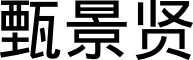
\includegraphics[scale=0.6]{YKY.png}}

\title{Reinforcement learning and quantum mechanics}
%\normalsize{-- a minimalist cognitive architecture combining\\
%reinforcement learning and deep learning}}
\titlerunning{Quantum mechanics}
\author{\usebox{\MyName} (King-Yin Yan)
% \\ \footnotesize{General.Intelligence@Gmail.com}
%\and
%Ben Goertzel
%\and
%Juan Carlos Kuri Pinto
}
\institute{General.Intelligence@Gmail.com}

\begin{document}

\maketitle

\setlength{\parindent}{0em}
\setlength{\parskip}{2.8ex plus0.8ex minus0.8ex}
% \setlength{\parskip}{2.8ex}

\begin{abstract}
	The Bellman equation governing dynamic programming (and reinforcement learning) is the discrete-time version of the Hamilton-Jacobi equation governing analytical mechanics.  This relation has been known for a long time.  If moreover we assume that ``states'' can be linearly superimposed on each other, this brings to mind the superposition of wave functions in quantum mechanics, governed by the Schr\"odinger equation.  The mysterious connection between Hamilton-Jacobi theory and Schr\"odinger theory was present from the very beginning of quantum mechanics (``the quantum-classical correspondence''), yet physicists are still unable to explain it to this day.
% 这篇是背景,介绍一个基於 \textbf{增强学习} 和 \textbf{深度学习} 的极简约的 cognitive architecture,它在数学上是一个Hamiltonian 系统,而其 Lagrangian 对应於智能系统的「奖励」或「欲望」的价值。 经典逻辑 AI 的技巧可以搬到这个 setting 之下,而连续时间化之后,可以用上微分几何的技巧。 传统的「逻辑 AI 知识表述」被新的表述法取代,后者的结构是由神经网络的深度学习「诱导」出来的。
%This is the first of a series of papers, introducing a minimalist cognitive architecture based on reinforcement learning and deep learning.  The system consists of an iterative function whose role is analogous to the consequence operator ($\vdash$) in logic.  It is fascinating to note this is a Hamiltonian system, whose Lagrangian corresponds to the value of ``desires'' or ``rewards'' for the intelligent agent;  but the usefulness of this idea is as yet unknown.  More importantly, the structure of classical logic-based AI can be transferred to the neural setting, the topic of our 2nd paper.
%Its continuous limit can be described by differential geometry.  The old-fashioned logic-based knowledge representation with discrete propositions is abandoned in favor of a representation induced by deep neural learning.
% The problem of general intelligence can be described and solved in the logic-based AI paradigm, but the main obstacle is that learning is too slow.  The logic-based knowledge representation with discrete propositions is abandoned in favor of a neural-based ``amorphous'' representation induced from the top down, using a deep neural network (DNN).  The DNN acts iteratively on a state space (the ``mental state''), forming a dynamical system.  This system is in turn controlled by reinforcement learning, ``navigating'' the space of mental states as in a maze.
\end{abstract}

%\begin{keywords}
%reinforcement learning, control theory, deep learning, cognitive architecture
%\end{keywords}

\setcounter{section}{-1}
\section{Bellman equation = Hamilton-Jacobi equation}
\label{sec:0}

Shortly after Bellman proposed his equation in 1953, Kalman recognized that its differential version is equivalent to the Hamilton-Jacobi equation of classical mechanics.

\begin{eqnarray}
\vcenter{\hbox{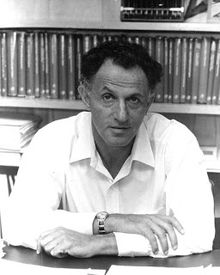
\includegraphics[scale=0.8]{Bellman.jpg}}} & \quad \quad & \vcenter{\hbox{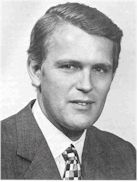
\includegraphics[scale=0.8]{Kalman.jpg}}} \\
\mbox{Richard E Bellman (1920-1984)} & \quad \quad & \mbox{Rudolf K\'{a}lm\'{a}n (1930-2016)} \nonumber
\end{eqnarray}

The \textbf{Bellman condition} says:  ``\uline{if we cut off a tiny bit from the endpoint of the optimal path, the remaining path is still an optimal path between the new endpoints}.''

Bellman equation (1953):
\begin{eqnarray}
& \mbox{\footnotesize value of entire path} \tikzmark{uEntire} \quad \quad \mbox{\footnotesize reward of choosing $\vect{u}$ at current state} \tikzmark{rCurrent} \quad \quad \mbox{\footnotesize value of rest of path} \tikzmark{uRest} \nonumber \\
\nonumber \\
& \boxed{\mbox{Bellman equation}} \quad \tikzmark{UEntire} U^*(\vect{x}) = \max\limits_{\vect{u}} \{ \; \tikzmark{RCurrent} R(\vect{u}) + \tikzmark{URest} U^*(\vect{x}_{t+1}) \; \}
\begin{tikzpicture}[overlay,remember picture]
  \draw (uEntire.center) +(-30pt,-3pt) -- ([shift={(4pt,12pt)}]UEntire.center);
  \draw (rCurrent.center) +(-80pt,-3pt) -- ([shift={(4pt,12pt)}]RCurrent.center);
  \draw (uRest.center) +(-65pt,-3pt) -- ([shift={(8pt,12pt)}]URest.center);
\end{tikzpicture}
\label{Bellman-eqn}
\end{eqnarray}
The meaning is that:  \uline{the difference in utility ($U$) of the current state compared with the next state is equal to the reward of the current state}.

Hamilton-Jacobi equation (1830's):
\begin{equation}
\boxed{\mbox{Hamilton-Jacobi}} \quad
\frac{\partial U^*}{\partial t} = - H
\label{Hamilton-Jacobi-eqn}
\end{equation}
This means that the differential in time of the utility ($U$) is the energy ($H$) of the current state.  ``Energy'' corresponds to instantaneous reward.

Simply put, \textbf{utility} is the integral of instantaneous \textbf{rewards} over time:
\begin{equation}
\boxed{\mbox{utility} $U$} = \int \boxed{\mbox{reward} $R$} \,dt
\end{equation}
%(价值有时用 $V$ 表示,但为避免和势能 $V$ 混淆故不用。)

%In \emp{control-theoretic} parlance, it is usually defined the \textbf{cost functional}:
%\begin{equation}
%\boxed{\mbox{cost } $J$} = \int L dt + \Phi(\vect{x}_\bot)
%\end{equation}
%where $L$ is the \textbf{running cost}, ie, the cost of making each step; $\Phi$ is the \textbf{terminal cost}, ie, the value when the terminal state $\vect{x}_\bot$ is reached.

In \emp{analytical mechanics} the \textbf{Lagrangian} ($L$) is a measure of energy and its time-integral is called the \textbf{action}:
\begin{equation}
\boxed{\mbox{action } $S$} = \int L dt
\end{equation}
% Hamilton's \emp{principle of least action} says that $S$ always takes the \textbf{stationary value}, ie, the $S$ value is extremal compared with neighboring trajectories.

Nothing new so far.

\section{Schr\"odinger equation}

Interestingly, if we want the ``mental state'' to be composed of a \textbf{superposition} of pure states, we may perform the \textbf{Fourier transform} on the pure states and add them together.  This immediately brings to mind the superposition of wave functions ($\Psi$) in quantum mechanics, in particular the Schr\"{o}dinger equation:
\begin{equation}
\boxed{\mbox{Schr\"{o}dinger}} \quad
i \frac{\partial \Psi}{\partial t} = \hat{H} \Psi .
\label{Schrodinger-eqn}
\end{equation}
Note that $\hat{H}$ is different from the $H$ in (\ref{Hamilton-Jacobi-eqn}).

This is very interesting because the Schr\"{o}dinger equation bears a close resemblance to the Hamilton-Jacobi equation, which has been recognized since the beginning of quantum mechanics, but no one has ever been able to elucidate this relation.  Bohm has made a controversial attempt at this goal, which we will discuss later.

\begin{eqnarray}
\vcenter{\hbox{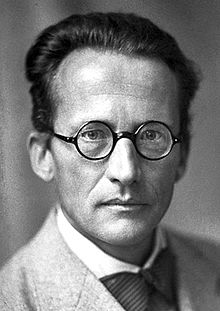
\includegraphics[scale=0.75]{Schrodinger.jpg}}} & \quad \quad & \vcenter{\hbox{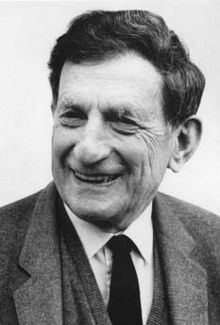
\includegraphics[scale=0.75]{Bohm.jpg}}} \\
\mbox{Erwin Schr\"{o}dinger (1887-1961)} & \quad \quad & \mbox{David Bohm (1917-1992)} \nonumber
\end{eqnarray}

Note:  the Schr\"{o}dinger equation can be written in this more ``physical'' form, with explicit dependence on position ($\vect{x}$) and time ($t$):
\begin{equation}
i  \hbar \frac{\partial}{\partial t} \Psi(x,t) = \left[ V(x,t) - \frac{\hbar^2}{2 m} \nabla^2 \right] \Psi(x,t) ,
\end{equation}
whereas the Hamilton-Jacobi-Bellman equation should be (in my opinion) dependent of the state $\Psi$:
\begin{equation}
\frac{\partial U(\Psi)}{\partial t} = - H(\Psi) .
\end{equation}

For example,
\begin{equation}
\english{I love you}
\label{love-single}
\end{equation}
is not a ``state'', but
\begin{equation}
\english{John loves Mary} \wedge \english{Mary loves Pete} \wedge \english{John is unhappy} \wedge ....
\label{love-affair}
\end{equation}
is a state.  That is because we take it that (\ref{love-affair}) completely describes a state of affairs in the \textbf{world}, whereas (\ref{love-single}) is just a partial description of a facet of the world.  In other words, the difference between a \textbf{state} and a \textbf{proposition}.  This distinction is quite obvious from the perspective of logic and reinforcement learning, but physicists might have overlooked it.

From the AI perspective, the meaning of $\Psi$ as ``state'' is clear, but the question is what is the meaning of $\vect{x}$, since the cognitive space is not physical space?  There may be several possibilities:
\let\labelitemi\labelitemii
\begin{itemize}
	\item Bohm's theory, which relates the Hamilton-Jacobi equation with Schr\"odinger's equation
	\item QFT (quantum field theory), \textbf{second quantization} and the creation / annihilation operators
	\item The Schr\"odinger equation is a kind of \textbf{linearization} of the Hamilton-Jacobi equation?
	\item There are many other quantization schemes:  path integral, group deformation, perturbative QFT, algebraic QFT, ....
\end{itemize}

\subsection{Bohm's theory}

The theory is developed and deepened by Bohm, Hiley, de Gosson, .... and others.
\begin{eqnarray}
\vcenter{\hbox{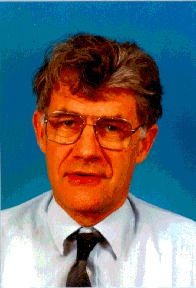
\includegraphics[scale=0.6]{Hiley.jpg}}} & \quad \quad & \vcenter{\hbox{
\includegraphics[scale=0.8]{de-Gosson.jpg}}} \\
\mbox{Basil J Hiley (1935-)} & \quad \quad & \mbox{Maurice de Gosson (1948-)} \nonumber
\end{eqnarray}

Starting from the Schr\"odinger equation for a single particle:
\begin{equation}
i \hbar \frac{\partial}{\partial t} \Psi = - \frac{\hbar^2}{2 m} \nabla^2 \Psi + V \Psi ,
\end{equation}
consider its polar-form solution:
\begin{equation}
\Psi(\vect{r},t) = R(\vect{r},t) e^{\frac{i}{\hbar} \Phi(\vect{r},t)}
\end{equation}
whose real and imaginary parts lead to:
\begin{equation}
\begin{cases}
\displaystyle R(\frac{\partial \Phi}{\partial t} + \frac{(\nabla_{\vect{r}} \Phi)^2}{2 m} + V) -  \frac{\hbar^2}{2 m} \nabla_{\vect{r}}^2 R = 0 
\vspace{0.7cm} \\
\displaystyle \frac{\partial R^2}{\partial t} + \mbox{div} (\frac{\nabla_{\vect{r}} \Phi}{m} R^2) = 0 .
\end{cases}
\end{equation}
The second equation is recognized as the continuity equation describing the time-evolution of a probability density:
\begin{equation}
\frac{\partial \rho}{\partial t} + \mbox{div} (\rho v) = 0
\end{equation}
whereas the first equation is recognized as the Hamilton-Jacobi equation:
\begin{equation}
\displaystyle \frac{\partial \Phi}{\partial t} + \frac{(\nabla_{\vect{r}} \Phi)^2}{2 m} + V -  \frac{\hbar^2}{2 m} \frac{\nabla_{\vect{r}}^2 R}{R} = 0 
\end{equation}
with a special Hamiltonian:
\begin{equation}
H^\Psi = H + Q^\Psi
\end{equation}
where
\begin{equation}
Q^\Psi = - \frac{\hbar^2}{2 m} \frac{\nabla_{\vect{r}}^2 R}{R}
\end{equation}
is known as the \textbf{quantum potential}.  $Q^\Psi$ is very much unlike a usual potential and is intrinsically \textbf{non-local}.  Its meaning is unclear (to me at least).

\subsection{Schr\"odinger equation = linearization?}

The \textbf{state linearization} of a dynamical system means to transform from the non-linear system:
\begin{equation}
\dot{\vect{x}} = \vect{f}(\vect{x}) % + \vect{g}(\vect{x}) \vect{u}
\end{equation}
to the (locally) linear system:
\begin{equation}
\dot{\vect{x}} = A \vect{x} + \vect{c} % + \sum g_i u_i
\end{equation}

The Schr\"odinger equation seems to be a particularly simple linear equation:
\begin{equation}
i \dot{\Psi} = \hat{H} \Psi
\end{equation}
where $\hat{H}$ is a linear operator.  Could it be that it is the linearized version of the Hamilton-Jacobi equation:
\begin{equation}
\dot{U}(\Psi) = - H(\Psi) \quad ?
\end{equation}
where we assumed that $U$ is expressed directly as a function of time.  If on the other hand $U$'s time-dependence is expressed through $\Psi$:
\begin{equation}
\dot{U} (\Psi) \dot{\Psi} = - H(\Psi) .
\end{equation}
\begin{equation}
\dot{\Psi} = - \frac{H(\Psi)}{\dot{U}(\Psi)} \quad ?
\end{equation}

\begin{tcolorbox}[colback=grey, breakable, enhanced] %_____________________________________

The \textbf{relativistic} Klein-Gordon equation:
\begin{equation}
\boxed{\mbox{Klein-Gordon}} \quad
- \frac{\partial^2 \Phi}{\partial^2 t} = (- \nabla^2 + m^2) \Phi
\end{equation}
appears to be 2nd-order in time, but that arised only because
\begin{equation}
E = \sqrt{\vect{p}^2 c^2 + m^2 c^4}
\end{equation}
and they had to deal with the operator $\vect{p}$ appearing within the $\sqrt{}$ sign.

Its original consideration is:
\begin{equation}
\frac{\partial \Phi}{\partial t} = E \Phi
\end{equation}
which has the same form as the Schr\"odinger equation.

\end{tcolorbox} %________________________________________________________________________

\subsection{Imaginary time $\rightsquigarrow$ stochastic processes}

When imaginary time is substituted into the Schr\"odinger equation, out pops the heat / diffusion equation:
\begin{equation}
\frac{\partial u}{\partial \tau} = D \Delta u .
\end{equation}

\section{Spectral theory}

\subsection{Fourier transform}

All of \textbf{transform theory} can be summarized as the following equation:
\begin{equation}
\boxed{\mbox{Transform theory}} \quad
y = \sum_n \langle \phi_n, y \rangle \phi_n
\end{equation}
where $\langle \phi_n, y \rangle$ represents the \textbf{analysis} stage where the input function is decomposed in terms of a basis set, and the entire $\sum$ represents the \textbf{synthesis} stage where the signal is reconstructed.

Hilbert created the spectral theory for \textbf{operators}:
\begin{eqnarray}
\vcenter{\hbox{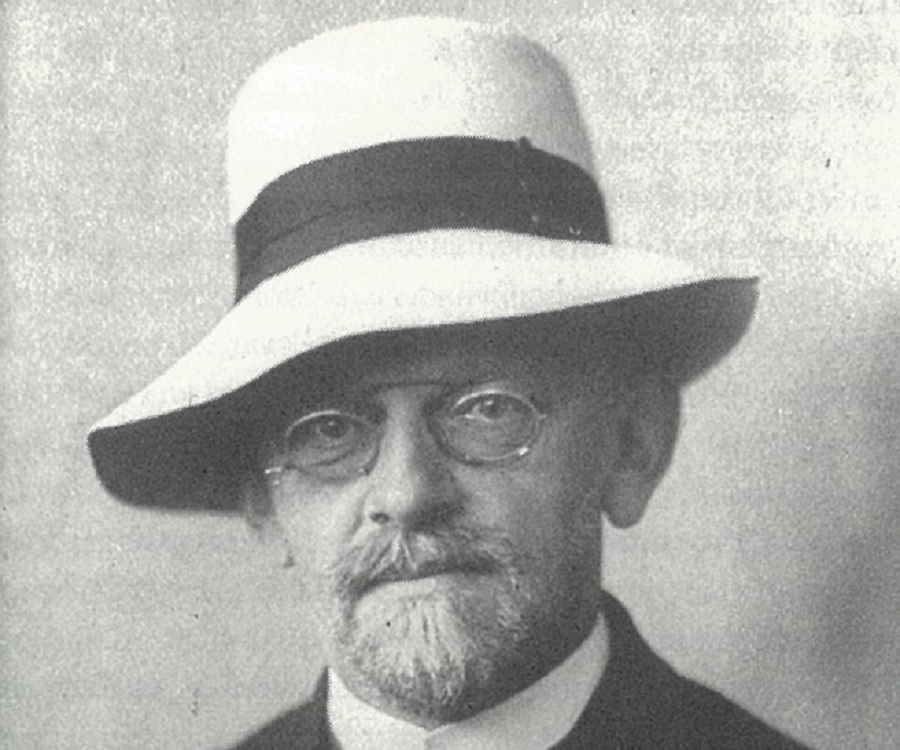
\includegraphics[scale=0.3]{Hilbert.jpg}}} \\
\mbox{David Hilbert (1862-1943)} \nonumber
\end{eqnarray}

\subsection{States and observables}

\subsection{Bra and ket notation}

\subsection{Lattice of projectors}



\section{Quantization (quantum field theory)}

\subsection{Creation and annihilation operators}

The \textbf{general scheme} for quantization is to factor the Hamiltonian as a product of 2 mutually adjoint operators:  \textbf{annihilation}, which lowers the energy level of $H$, and \textbf{creation}, which raises the energy level.  These 2 operators completely describe the \textbf{spectrum} of $H$.

Starting from the classical Hamiltonian of a single particle with mass $m$ and charge $e$ interacting with an electromagnetic field with vector potential $\vect{A}$ and scalar potential $\phi$:
\begin{equation}
H = \frac{1}{2 m} (\vect{p} - e \vect{A})^2 + e \phi ,
\end{equation}
invariance under gauge transformations dictates that:
\begin{equation}
\nabla^2 \vect{A} - \frac{\partial^2 \vect{A}}{\partial t^2} = 0
\end{equation}
whose general solution is:
\begin{equation}
\vect{A}(\vect{x}, t) = (\frac{1}{2 \pi})^2 \int d^3\vect{k} d\omega \sum_{\lambda = 1}^{2} a_{\lambda}(\vect{k}) e^{i (\vect{k} \cdot \vect{x} - \omega t)} \vect{\epsilon}_{\lambda}(\vect{k}) \delta({k^2}) .
\end{equation}
This can be seen as a \textbf{Fourier transform} of $\vect{A}$.

\section{Tropical geometry}

\begin{equation}
(\times, +) \rightarrow (+, \max)
\end{equation}

\begin{eqnarray}
x \oplus y    &=& \log (t ^x + t^y) \nonumber \\
x \otimes y &=& x + y
\end{eqnarray}


\section{Q-learning}

In AI reinforcement learning there is an oft-employed trick known as $Q$-learning.  $Q$ value is just a variation of $U$ value;  there is a $U$ value for each state, and $Q$ is the \textbf{decomposition} of $U$ by all the actions available to that state.  In other words, $Q$ is the utility of doing action $\vect{u}$ in state $\vect{x}$.  The relation between $Q$ and $U$ is:
\begin{equation}
U(\vect{x}) = \max\limits_{\vect{u}} \, Q(\vect{x}, \vect{u})
\end{equation}
The advantage of $Q$ is the ease of learning.  We just need to learn the value of actions under each state.  This is so-called ``\textbf{model free learning}''.

%The \emp{Bellman equation} governs reinforcement learning just as in control theory:
%\begin{eqnarray}
%\boxed{\mbox{optimal path}} = & \mbox{choose max reward on current path segment} \nonumber \\
%& \quad + \boxed{\mbox{the rest of optimal path}}
%\end{eqnarray}
%In math notation:
%\begin{equation}
%U^*_t = \max_{u} \{ \; \boxed{\mbox{reward}(u, t)} + U^*_{t-1} \; \}
%\end{equation}
%where $U$ is the ``long-term value'' or \emp{utility} of a path.

%Conceptually, $U$ is the \textbf{integration} of instantaneous rewards over time:
%\begin{equation}
%\boxed{\mbox{utility, or value} U} = \int \boxed{\mbox{reward} R} \,dt
%\end{equation}

\subsection{Actions = cognitive state-transitions = ``thinking''}

In our system there are 2 things that need to be learned:
\begin{enumerate}
\item The transition function $\vect{F}: \vect{x} \mapsto \vect{x}'$.  $\vect{F}$ represents the \textbf{knowledge} that constrains thinking.  In other words, the learning of $\vect{F}$ is the learning of ``static'' knowledge.
\item Find the optimal trajectory of the state $\vect{x}$.  This corresponds to optimal ``thinking'' under the constraints of static knowledge.
\end{enumerate}
\begin{equation}
\vcenter{\hbox{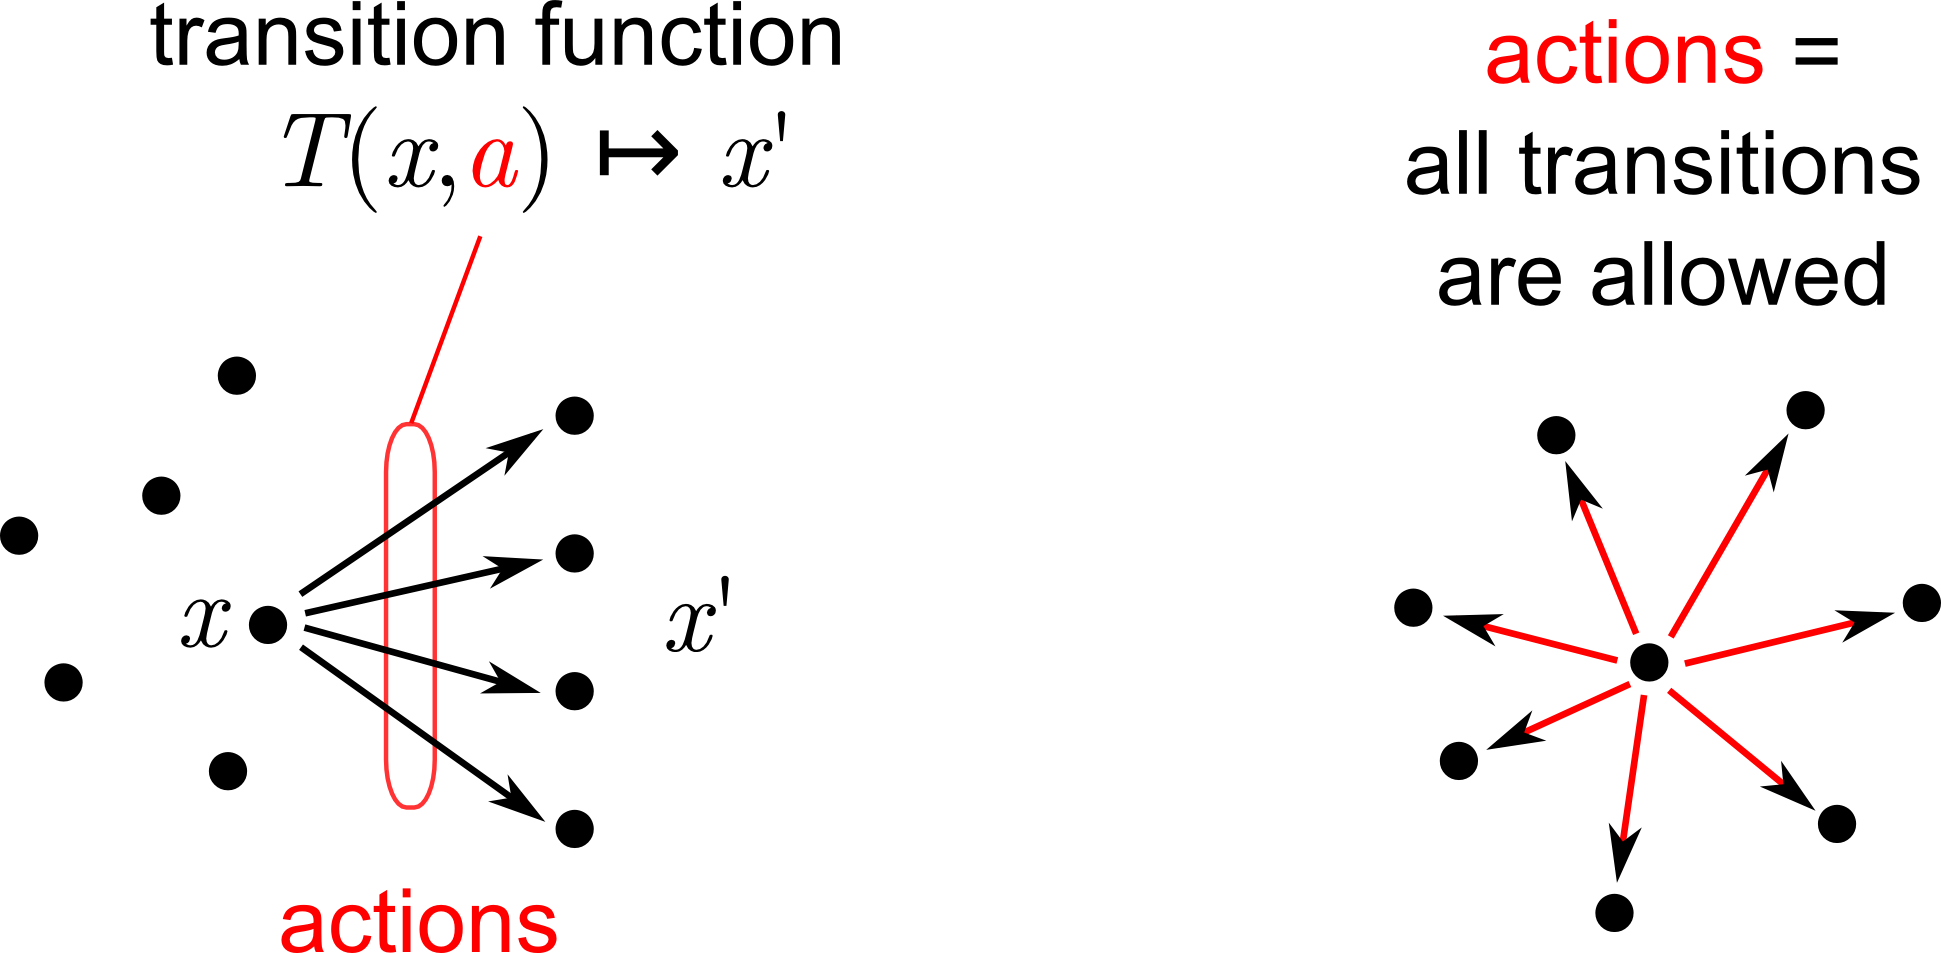
\includegraphics[scale=0.7]{Q-learning-2-views.png}}}
\end{equation}
In traditional reinforcement learning (left view), the system chooses an action $\vect{a}$, and the transition function $\vect{F}$ gives the probability of reaching each state $\vect{x}_i$ given action $\vect{a}$.  In our model (right view), all possible cognitive states are potentially \textbf{reachable} from any other state, and therefore the action $a$ coincides with the next state $x'$.

\begin{comment}
%==================================================================================
Under the reinforcement learning framework, intelligence is decomposed into \textbf{thinking} and \textbf{learning}:
\begin{itemize}
\item \emp{Thinking} means finding the optimal trajectory of $\vect{x}$ according to the \textbf{knowledge} stored in the deep NN.  This is achieved using the Bellman equation to calculate $\vect{u}^*$.  The trajectory of $\vect{x}$ is constrained by the deep NN (in other words, the system must think in accordance with \textbf{correct knowledge}).  While thinking, the deep NN stays \textbf{constant}.

\item \emp{Learning} means learning the weights in the deep NN.  Changing $W$ changes $\vect{F}$, which determines the state equation (\ref{eqn0}), so the entire system becomes a new one.  In other words, deep NN learning is a kind of \textbf{second-order learning}:  Consider 2 systems $\vect{F}$ and $\vect{F} + \epsilon \hat{\vect{F}}$, after \uline{many trials} of thinking with different premises, if the average reward is higher in the altered system, $\vect{F}$ will learn towards the $\hat{\vect{F}}$ direction.
% 即是根据已学得的\textbf{知识}(知识储存在 deep NN 里),在思维空间中找寻 $\vect{x}$ 最优的轨迹,方法是根据 Bellman 方程计算 $\vect{u}^*$。 $\vect{x}$ 的轨迹受 deep NN 约束(亦即是说,系统只能依据\textbf{正确的知识}去思考),思考时 deep NN 是\textbf{不变}的。
%\item \emp{学习}就是学习神经网络 deep NN 的 weights $W_\ell$,改变 $W$ 即改变 $\vect{F}$,而$\vect{F}$ 决定\textbf{状态方程} (\ref{eqn0}),所以整个系统变了另一个系统。 换句话说,deep NN 的学习是一种 \textbf{second-order learning}: 考虑两个系统 $\vect{F}$ 和 $\vect{F} + \epsilon \hat{\vect{F}}$,经过很多次思考过程,如果奖励的平均值在后者有所增加,则 $\vect{F}$ 向 $\hat{\vect{F}}$ 方向学习。
\end{itemize}
%==================================================================================
\end{comment}

\begin{comment}
%==================================================================================
\section{Deep learning}

The combination of deep learning with reinforcement learning, ie deep reinforcement learning (DRL), is very powerful.  For example, DRL is able to play Atari games to human levels \cite{Mnih2013}.  Their architecture is depicted in this diagram:
\begin{equation}
\vcenter{\hbox{\includegraphics[scale=0.5]{Atari-Q-learning.jpg}}}
\end{equation}

Recall our main architecture:
%\begin{equation}
%\vcenter{\hbox{\includegraphics[scale=0.5]{genifer-model-0.png}}}
%\end{equation}

The ``transition function'' neural network can also take an \textbf{action} parameter $u$:
%\begin{equation}
%\vcenter{\hbox{\includegraphics[scale=0.5]{model-with-u.png}}}
%\end{equation}
But such a neural network requires a novel learning algorithm that is \textbf{reward-driven} rather than the traditionally \textbf{error-driven} back-propagation.  Such an algorithm is difficult to design because it cannot rely on old-fashioned gradient descent.

One solution that avoids the difficulty is to make the neural network compute the Q-value:
%\begin{equation}
%\vcenter{\hbox{\includegraphics[scale=0.5]{model-Sayaka.png}}}
%\end{equation}
This means that we can compute $Q$ for any transition $x \stackrel{u}{\mapsto} x'$.  During the ``action'' (ie, ``thinking'') stage, we hold $x$ fixed, and search for $(u, x')$ that maximizes $Q$;  This can be done by \textbf{stochastic gradient descent}.  During the ``learning'' stage, we are given certain transitions $(x, u, x')$ and we train the neural network to adjust $Q$ via standard \textbf{Bellman update}.

%==================================================================================
\end{comment}

% ================================== comment out ==================================
\iffalse

From the viewpoint of reinforcement learning, we aim to learn the \emp{policy} function: \par
\begin{equation}
\begin{tikzcd}[]
\mbox{policy : ~~state} \arrow[r, mapsto, "\scalebox{0.8}{action}"] & \mbox{state'}
\end{tikzcd}
\end{equation}
Where $K$ can be regarded as the \emp{mental state}, and thus an \emp{action} in RL turns $K$ into $K'$.

In our system, there are 2 pathways that act on $K$, via RNN and RL respectively: \par
\begin{equation}
\begin{tikzcd}[column sep=huge]
& K'_1 \arrow[dd, dashed, no head, "\scalebox{1.3}{$\approx$}"] \\
K \arrow[ur, "\mbox{RL}"] \arrow[dr, "\mbox{RNN}"'] & \\
& K'_2
\end{tikzcd}
\end{equation}
In RL, the action $a$ acts on $K$, whereas in RNN, $R$ acts on $K$.

\emp{Note}: RNN and RL are learning algorithms, and if they are both applied to the same problem, conflicts will necessarily arise, unless there is a way to combine them.

At state $K$, we estimate the Q-value $Q(K \stackrel{a}{\mapsto} K')$.  The action that would be chosen at state $K$ is $\displaystyle \arg\max_a Q(K \stackrel{a}{\mapsto} K')$.  This could be used to train the RNN via $\displaystyle K \vdash_W ...^n K'$.

RL 在众多状态 $K$ 之间游荡,学习 $Q(K \mapsto K')$。  因为 RL 独有奖励讯息,我们必需用 RL 来教导 RNN 学习,反之不可。  第一个问题是: RL 如何在 $K$ 之间游荡?   游荡是随机的,但也可以借助 RNN 的随机性、或在 RNN 自身的游荡中注入更多随机性、或者根本就是 RL 自己产生的随机性。  接下来的问题是: RNN 如何用 $Q$ 值来诱发学习?

RNN 的 ``$n$-fold'' 学习可以通过以下方式实现: 
\begin{itemize}
\item stochastic forward-backward propagation
\item genetic?
\item 最有趣的是 Hebbian learning,因为它似乎特别适合这情况。  
\end{itemize}

RNN 的本质是什么?  它似乎是一个 recurrent hetero-associative memory。  但其实它还需要将 input 作类似於 Word2vec 的 encoding。  这个 encoding 将「相似」的思维状态 $K$ 归到同类。  利用空间中的相似度,RL 可以用一些连续函数来近似 Q 值(详细情况还有待分析)。

另一个问题是: 虽然用函数的近似可以做到 generalization,但另一个方法是利用状态 $K$ 中的空位作暂时储存。 这两者似乎很不同。  问题似乎在於: 状态转换 $K \mapsto K'$ 是不是对应於逻辑中的\emp{一条} rule?  答案似乎是 yes。  这个共识是很重要的。  如果用 decision tree,需要的是向量空间中的相似度。

现在的关键是「状态变量」。  因为它可以做到符号逻辑中靠变量的 generalization,这是前所未有的。  这种 generalization 似乎不需要相似度,因为它是符号的!  会不会在向量空间中的状态变量 能够做到之前逻辑变量做不到的动作?  不管怎样,用 RNN 学习这些变量的动作似乎是很难的,因为这些动作似乎不是对\emp{误差}的梯度下降。  除非这些动作本身也近似於其他动作,但那是怎样的近似?  学习 multi-step logic 其实和以前的 forward / backward chaining 没有分别!  唯一分别是命题的 representation 改变了,它未必像符号的 concatenation。  所以问题仍然是 ``$n$-fold'' 学习法。 

而且注意: RL 的 generalization 根本上不同於 rules 空间中的 generalization。 前者是思维空间 $K$ 中的一般化,后者也可以是 $K$ 空间的一般化,但也可以是依赖「状态变量」的一般化。

一般来说,RL 和 RNN 的行动和学习,是可以互相独立的。  

还有 heterarchical 的分类法。  想用 decision tree 或什么,达到不同网络的\emp{分工}。  在组织知识这方面,深度网络有没有用?  可以想像,在视觉识别中,在网络的最上层有很多 objects,而它们都可以还原到底层的 features。  网络有更多层,可以识别的事物更抽象。  但现在我们要的不是\emp{模式识别},而是 mapping。 特别是抽象模式的 mapping。  想要的是: 大量的 rules,将不同的 $K$ 映射到新的 $K'$。

还有一点要澄清的是: 究竟每一个「思元素」在向量空间中是不是\emp{一点}?  如果有了这个「思元素 = 点」假设,则每次 iteration 应该会删除一个思元素,而用另一个(全新的)思元素取代之。  这样,$K \mapsto K'$ mapping 就有了更确定的结构。  这样的 setup 已经很接近 logic 系统,但其学习算法仍然很有 combinatorial 的 ``feel''。 (因为只有当两个 rules 串连之后,才能达到某个结论,而这个串连有没有中间的 continuous 状态?)  这种串连通常是怎样找到的?  

现在有一转机: 如果「思元素 = 点」,则「状态变量」的形成似乎会很普遍,而我们可以集中研究如何学习 single-step rules。 RL 的 rewards 可以指导学习,但这些「终极 rewards」对学习的细节没有指导作用。  我们似乎可以用「\emp{时间延迟}」来达到「状态变量」的效果,这个做法无形中增加了使用状态变量的机会。  

现在总结一下仍然有待回答的问题:
\begin{itemize}
\item RL 的 generalization 如何做?
\item iterative thinking map 如何 learn?
\item 
\end{itemize}

Hebbian 的情况是: 有某一 I/O pattern; 我想 strengthen 这 pattern。 

Assuming the learning is correct, $K'_1$ and $K'_2$ should be roughly the same \textemdash~ but this ignored the possibility that one path may take multiple steps to converge with the other path.  \footnote{This situation has been encountered in term rewriting systems (TRS):  If in a TRS any 2 different rewriting paths always converge to the same result, it is said to have the \emp{Church-Rosser property}.  For example the $\lambda$-calculus invented by Church has this property.} 

Now I stipulate that $R$ be more ``refined'', that is to say, applying $D^n$ times may be equivalent to applying $a$ once:
\begin{equation}
\begin{tikzcd}[column sep=huge]
& K'_1 \arrow[dd, dashed, no head, "\scalebox{1.3}{$\approx$}"] \\
K \arrow[ur, "\scalebox{1.3}{$a$}"] \arrow[dr, "{\scalebox{1.3}{$D^n$}}"'] & \\
& K'_2
\end{tikzcd}
\end{equation}
Using a different notation, $a$ is the \emp{restriction} or \emp{section} of $D^n$ at point $K$: $a = D^n|_K$.

Now the question is, do the RNN and RL paths have any \textit{essential} difference?
\begin{itemize}
\item Their internal \emp{representations} are different:\par
\dashh RNN is a multi-layer neural network\par
\dashh RL's representation is $Q(\mbox{state},\mbox{action})$, usually stored as a \textit{look-up table}, although $Q$ could be approximated by a neural network as well.
\item RL learns through \emp{rewards}, RNN learns from \emp{errors}.  Thus RL has broader applicability, because not all questions have ``correct answers'' that could be measured by errors.  In RL we just need to praise Genifer whenever she displays good behavior.
\item The internal cognitive state $K$ exists because of RNN:  it is simply the vector input and output of the RNN.  Without this $K$, RL would be clueless as to what are its internal states.  It can be said that the RNN provides a \textit{machinery} for RL to control.
\end{itemize}

% programming needed:
% RNN: with special back-prop
% RL: approximate Q(K,a), using special NN that can find max also

% 整体来说,RL 可以操控的 actions 包括:
% \begin{enumerate}[\tab (A)]
% \item apply $K \stackrel{D}{\mapsto} K'$ \par
% 但注意: $K$ 是认知状态,$R$ 是对 $K$ 进行「合乎逻辑的推论」。 所以,无论发生什么事,我们都会将 $R$ 作用在 $K$ 上几次。 换句话说,$R$ 是\ds{必然}进行的动作,或者可以看成是在\ds{背景}下进行的运作,所以不需要用 RL 学习。 %RL 的用处是学习如何在很多 actions 之间选择最好的一个,所以 $R$ 不是 RL 需要学习的 action,它只是。

% \item 改写认知状态 $K \mapsto K'$ \par
% RL 的 actions (A) 是
% 在思考过程中改变 $K$ 的值。 例如我们得到一个局部结论,这个局部结论的状态不是最终答案,但也比什么都没有的效用更高。 改写 $K$ 的方法可以是: 例如 将 $K \mbox{ += } \delta K$,或者 「if $K \in$ 某 region,then $K \mbox{ += } \delta K $」。

% \item 学习: change $R$ \par

From the perspective of reinforcement learning, we could reward some results of multi-step inference: \par
\begin{equation}
\begin{tikzcd}[row sep=tiny]
K_0 \arrow[r, mapsto, "\scalebox{1.3}{$a$}"] & K_\vdash \quad \updownarrow \bigstar
\end{tikzcd}
\end{equation}
$\updownarrow \bigstar$ means ``to give positive or negative rewards''.  We want to learn $a$ which is the action to be taken at state $K$.  The learning algorithm is based on the famous \emp{Bellman optimality condition} (see next section).

Perhaps we should use RL to \textit{guide} the learning in RNN, as RNN is more fine-grained....

To combine the 2 learning approaches, we could use the technique of \emp{interleaving}: for each step apply RL once, apply RNN $n$ times.

% 但 $R$ 本身是 RNN,它还可以透过 back-prop 进行学习,两者似乎是不同的。  Back-prop 是透过 $\frac{\partial}{\partial D}(\mbox{error})$ 的梯度来学习。

The learning in RNN may also involve \emp{neurogenesis} (adding new neurons and connections), but I have not considered this aspect yet.

% RNN 的 $R$ 也是将 $K$ 变成 $K'$ 的作用:\par
%\begin{figure}[h]
%\centering
%\begin{tikzcd}[row sep=tiny]
%K \arrow[r, mapsto, "\scalebox{1.3}{$R$}"] & K'
%\end{tikzcd}
%\end{figure}
% $R$ 和 RL 的 actions 是不一样的。

There are 4 learning modes:
\begin{itemize}
\item learning to listen/talk
\item RL-based learning
\item inductive learning
\end{itemize}

\section{Misc points}

\begin{itemize}
\item If sigmoid is replaced by polynomial, universal approximating property may be retained.

\item Banach fixed point theorem does not apply because $R$ in general need not be contractive.  Question is whether $R$ necessarily converges to fixed points and the answer is no.

\item If reasoning operator $R$ is continuous, the flow of the dynamical system is governed by an autonomous differential equation.  Poincare-Bendixson only applies to dynamical systems on the plane, and is irrelevant to systems whose phase space has dimension $\geq 3$, or to discrete dynamical systems.

\item Time can be discrete or continuous.

\item Goal is to find minimizer of error (ie, to approximate a function given some input-output data points).  The (finite) set of local minima can be solved via setting $\frac{\partial R}{\partial W} = 0$.  The number of local minima can be calculated as: ?  McClelland paper.

\item If operator is discontinuous, what advantages can be gained?
\end{itemize}

What I want to do now is to determine if $R$ implemented as a deep network is sufficient to model human-level reasoning.

One principle seems to be that logical conclusions must not proliferate indefinitely.  But we are not sure what kind of structural constraints this would impose on the vector space.  Or whether we should impose such constraints manually.

What other properties are desired for the implementation of $R$?

\section{Architecture}

First, cartoon version:
\begin{equation}
\vcenter{\hbox{\includegraphics[scale=0.5]{architecture-cartoon.png}}}
\end{equation}

\begin{equation}
\vcenter{\hbox{\includegraphics[scale=0.5]{RNN-topology.png}}}
\end{equation}

TO-DO:  The state space $X$ may be too large and we may need an \emp{attention mechanism} to select some parts of $X$ for processing by $R$.  This is the notion of \emp{working memory} in cognitive science.
\begin{equation}
\vcenter{\hbox{\includegraphics[scale=0.4]{working-memory.png}}}
\end{equation}

\section{Deep Recurrent Learning}

The learning algorithm for $R$ is central to our system.  $R$ learns to recognize input-output pairs $( \vec{x}_0, \vec{x}^* )$.  What makes it special is that $R$ is allowed to iterate a \textit{flexible} number of times before outputting an answer.  In feed-forward learning we simply learn single-pass recognition, whereas in common recurrent learning we train against a \textit{fixed} time sequence.  Here, the time delay between input and output is allowed to stretch arbitrarily.

Suppose the recurrent network $R$ iterates $n$ times:
\begin{equation}
\vec{x}_{t+1} = \overbrace{R \circ R \circ ...}^{n} (\vec{x})
\end{equation}

As $n \rightarrow \infty$, we get the continuous-time version (a differential equation):
\begin{equation}
\frac{d\vec{x}(t)}{dt} = \mathfrak{R}(\vec{x}(t))
\end{equation}

We could run the network $R$ for a long enough time $T$ such that it is highly likely to reach an equilibrium point.  Then:
\begin{equation}
\vec{x}_{T} = \int_0^T \mathfrak{R}(\vec{x}(t)) dt
\end{equation}
and the error:
\begin{equation}
\mathscr{E} = \vec{x}^* - \vec{x}_{T}
\end{equation}
where $\vec{x}^*$ is the target value which is independent of time.
\begin{eqnarray}
\frac{\partial\mathscr{E}}{\partial\vec{W}} &=& - \frac{\partial}{\partial\vec{W}} \int_0^T \mathfrak{R}(\vec{x}(t)) dt \nonumber \\
&=& - \frac{\partial}{\partial\vec{W}} \int_0^T \sigmoid(W_1 \sigmoid(W_2 ... \sigmoid(W_L \vec{x}(t))) dt
\end{eqnarray}

When there are many layers or if the recurrence is too long, back-prop learning becomes ineffective due to the \emp{vanishing gradient} problem.  One solution is to use the \emp{rectifier} activation function:
\begin{equation}
\rectifier (x) = 
\begin{cases}
x, & \mbox{if } x \geq 0 \\
0, & \mbox{otherwise}
\end{cases}
\end{equation}
Since its derivative is piecewise constant, it does not suffer from the vanishing gradient problem.

\subsection{Forward-backward Algorithm}

This is inspired by forward- and backward-chaining in LBAI.  We propagate the state vector from both the initial state $\vec{x}_0$ as well as the final state $\vec{x}^*$.  This bi-directional propagation is added with noise and repeated many times, thus implementing a \emp{stochastic local search}:

\begin{equation}
\vcenter{\hbox{\includegraphics[scale=0.6]{forward-backward-algorithm.png}}}
\end{equation}

When the forward and backward states get close enough, a successful path is found, and we record the gap and the noises along the path, and use them to train $R$ so that this new path would be recognized.

% One key question is how to deal with "don't care" bits?  One answer is that their errors are zero.  But then this is the same as the error for "correct" weights, which seems not well.  There's got to be a way to alter weights when the answer is correct...

% For \# Iteration = 0, output is immediately known, so potentially the training can be done.  But how to convey that all these alterations of weights are \emp{optional}?

% \section{Reinforcement learning}

% ================================== comment out ==================================
\fi

\bibliographystyle{plain} % or number or aaai ...
\bibliography{AGI-book}

\end{document}
